%File: formatting-instruction.tex
\documentclass[letterpaper]{article}
\usepackage{aaai}
\usepackage{times}
\usepackage{helvet}
\usepackage{courier}

\usepackage{amsmath}
\usepackage{amsfonts}
\usepackage[utf8]{inputenc}
\usepackage{amsmath,amssymb}
\usepackage{array}
% \usepackage{xcolor}
\usepackage{graphicx}
\usepackage{multirow}
\usepackage{subfig}
\usepackage{todonotes}
\usepackage{listings}
\usepackage{makecell}
% \usepackage[table,xcdraw]{xcolor}
\lstset{
  frame=tb,
  aboveskip=3mm,
  belowskip=3mm,
  showstringspaces=false,
  columns=flexible,
  basicstyle={\small\ttfamily},
  breaklines=true,
  breakatwhitespace=true,
  tabsize=3
}

\frenchspacing
\setlength{\pdfpagewidth}{8.5in}
\setlength{\pdfpageheight}{11in}
\pdfinfo{
/Title (Progress Report I: Leveraging Large Language Models for Creative Story Generation)
/Author (Yuetian Chen, Yiyang Cai, and Brendan Capuzzo)}
\setcounter{secnumdepth}{0}  
 \begin{document}
% The file aaai.sty is the style file for AAAI Press 
% proceedings, working notes, and technical reports.
%
\title{Progress Report I: \\ Leveraging Large Language Models for Creative Story Generation}
\author{Group U1: \{Yuetian Chen, Yiyang Cai, and Brendan Capuzzo\}\\
ML and Optimization - CSCI 4968 - 01, Spring 2023\\
\{cheny63, caiy3, capuzb\}@rpi.edu\\
}
\maketitle
\begin{abstract}
\begin{quote}
Creative story generation is a challenging and intriguing task in the field of natural language processing. With the advent of Large Language Models (LLMs), there is growing interest in utilizing their impressive text generation capabilities for generating coherent and engaging stories. In this progress report, we present our ongoing research project that aims to leverage LLMs, such as T5, for creative story generation by exploring novel techniques for narrative structure generation. Our primary objective is to develop a framework that generates stories with rich narrative structures, including character development, plot progression, and conflict resolution. We discuss our methodology, which involves using knowledge graphs, text planning techniques, and fine-tuning to improve story generation. Preliminary results indicate that our approach shows promise in generating coherent and engaging stories, and our future work will focus on refining the framework and evaluating its effectiveness in producing creative and captivating stories.
\end{quote}
\end{abstract}

\section{Introduction}
Storytelling is a fundamental aspect of human culture, allowing us to communicate, entertain, and educate. With the advent of artificial intelligence and natural language processing, the possibility of generating creative and engaging stories automatically has become an exciting research area. Large Language Models (LLMs), such as GPT-3 and T5, have demonstrated impressive capabilities in generating human-like text, making them promising candidates for creative story generation.

In this progress report, we provide an update on our research project, which focuses on investigating the potential of LLMs for creative story generation. Our primary objective is to improve the framework that leverages the text generation capabilities of LLMs and combines them with novel techniques for narrative structure generation. This would allow the generation of coherent and engaging stories that encompass rich narrative structures, including character development, plot progression, and conflict resolution. As shown in Table~\ref{storyExampleII}, for language model with fewer parameter, this is never a easy task.

\begin{table}[h]
    \centering
    \begin{tabular}{p{0.45\linewidth}|p{0.45\linewidth}}
    \textbf{expected}                & \textbf{actual [\texttt{T5$_{base}$}]}                \\ \hline
    Mary had been feeling depressed lately.                        & Mary had been feeling depressed lately. \\ \hline
    she decided to go see a psychiatrist.                          & She decided to go to a psychiatrist.    \\ \hline
    Psyched, her psychiatrist diagnosed her with depression and sent her to see. & She was diagnosed with schizophrenia. \\ \hline
    Medicant took her to get an antidepressant and prescribed her. & She was very happy.                     \\ \hline
    Thankfully it eventually made her feel better again.           & She was very happy.                    
    \end{tabular}%
    \caption{An example comparing the baseline model and model with emotion and keywords prompting}
    \label{storyExampleII}
\end{table}

To achieve this goal, we have been working on several tasks, including understanding the current state of the art in story generation, analyzing the strengths and limitations of existing LLMs, and exploring various techniques for generating narrative structures. In the following sections, we will discuss our methodology, preliminary work, and the progress we have made thus far in our project.

\section{Literature Review}
Automatic story generation has long been a challenging task in natural language processing, and such efforts date back to the 1970s~\cite{Meehan1977TALESPINAI}. Earlier attempts, such as symbolic planning systems~\cite{Riedl_2010}, utilize planning techniques to create plausible and coherent plots for stories. In addition, case-based or analogical modeling systems generate new narratives based on adapted existing stories~\cite{Gervs2005StoryPG}. However, while these approaches can create stories with impressive coherence and consistency, they often require extensive knowledge engineering and restrict to a limited domain. To address the issue, large crowd-sourced corpora of stories are used to help generate stories~\cite{10.1145/2362394.2362398,Li}. Modern approaches based on neural language models have been explored to generate plot-driven stories~\cite{fan-etal-2018-hierarchical}.
Moreover,~\cite{yang-etal-2019-enhancing-topic} incorporates commonsense knowledge into the generator using a novel memory mechanism and utilizes adversarial training to improve the diversity and originality of essay generation.~\cite{Tambwekar2019ControllableNS} leverages reward strategies during the generation to guide the language model toward generating a coherent story.~\cite{Liu_Li_Yu_Huang_Liu_Zhao_Yan_2020} proposes a character-centric story-generation model that can produce stories consistent with characters' profiles. 

In contrast to previous work, we propose an interactive visual story generation pipeline in which the user can specify keywords and emotions that will appear in the next sentence. The system generates the sentence and associated images for the user based on this information.

\section{Methodology}
In this section, we provide an in-depth overview of the methodology utilized in our research project, which focuses on creative story generation using Large Language Models (LLMs) such as T5. Our approach is built on a foundation of three key components: LLM fine-tuning, knowledge distillation, and parameter-efficient fine-tuning (PEFT). These components work in tandem to create a comprehensive framework that generates engaging stories with rich narrative structures.

\textbf{LLM Fine-tuning:} The first component of our methodology involves fine-tuning pre-trained LLMs on a dataset specifically created for the purpose of creative story generation. This dataset includes a diverse selection of high-quality stories, covering a wide range of themes, genres, and narrative styles. The fine-tuning process enables the LLM to learn the nuances of creative storytelling, including character development, plot progression, and conflict resolution. By adjusting the model's parameters and employing various optimization techniques, we aim to maximize the performance of the fine-tuned model in generating creative stories.

\textbf{Knowledge Distillation:} The second component of our approach is knowledge distillation, which is employed to condense the information acquired during the fine-tuning process into a smaller, more manageable model. This process involves training a compact model to mimic the output distribution of the larger, fine-tuned model. As a result, the distilled model retains most of the original model's capabilities while offering the advantages of reduced computational requirements and faster generation times. This streamlined model is better suited for practical deployment in creative story generation tasks.

\textbf{Parameter-Efficient Fine-Tuning (PEFT):} The third component of our methodology is the incorporation of Parameter-Efficient Fine-Tuning (PEFT). This technique is designed to optimize model performance and computational efficiency by fine-tuning only a subset of the model's parameters that are deemed most relevant to the creative story generation task. By carefully selecting and adjusting these critical parameters, we can achieve improved performance with fewer computational resources. The PEFT process enables us to create a more efficient model for generating creative stories without compromising the quality of the output.

Together, these three components form the core of our research project's methodology, which aims to harness the power of Large Language Models for creative story generation. By fine-tuning, distilling, and applying parameter-efficient techniques, we strive to develop a robust and efficient framework capable of producing captivating and imaginative stories.
% \subsection{LLM Finetuning}
% \subsection{Knowledge Distilation}
% \subsection{Parameter-Efficient Fine-Tuning (PEFT)}
\section{Data Availability}
In our project, we aimed to create a diverse and comprehensive training dataset for fine-tuning the language model on creative story generation tasks. To achieve this, we combined the stories from both the ROCStories dataset and the WritingPrompts dataset. We denote this combined dataset as $\mathbf{S_{total}}$ hereinafter. Also, we applied various ways to visualize the information in the original story and used tags to visualize them. This section will be highlighted in the last two subsections
\subsection{ROCStories}
The ROCStories dataset~\cite{mostafazadeh2016corpus} serves as a significant resource for researchers and practitioners in the field of natural language processing, particularly for commonsense story understanding and generation tasks. Comprising 98,161 five-sentence stories, the ROCStories dataset focuses on simple, everyday events. The stories were carefully curated through a crowdsourcing approach and subjected to rigorous review to ensure both quality and consistency. The dataset's primary purpose is to evaluate a model's ability to understand and generate narratives by examining its capacity to capture various aspects of commonsense reasoning. These aspects include understanding causal and temporal relationships, interpreting characters' emotions, and discerning their intentions.

Each story within the ROCStories dataset consists of five sentences. The first four sentences describe the story's events, while the fifth sentence provides a conclusion. A common application of the dataset is in a cloze test format, in which models are given the initial four sentences and tasked with predicting the fifth sentence or suggesting a reasonable alternative.

As a benchmark for a wide range of natural language understanding and generation tasks, such as story completion, commonsense reasoning, and language modeling, the ROCStories dataset has proven to be an invaluable resource. Researchers employ the dataset to assess and compare the performance of various models and techniques, allowing for the development of increasingly sophisticated models in the realms of story understanding and generation. The ROCStories dataset continues to facilitate advancements in natural language processing, contributing to the ongoing development and improvement of language models.
\subsection{Writing Prompts}

The writing prompts dataset is a robust set of data that is important for research in natural language processing and is highly beneficial to the area of story generation. This dataset consists of 303,358 pairs of writing prompts and human-written stories. The writing prompts are taken from an online forum, specifically the Reddit  \texttt{r/WritingPrompts} forum\footnote{https://www.reddit.com/r/WritingPrompts/}. Each of the writing prompts has a human-generated story associated with it. The prompts act as the input and the independent variables of the dataset. The stories are the dependent variables and act as the result of the prompt. The dataset is scraped from the online forum so it focuses on an array of diverse topics, lengths, and ideas. Reddit, the online forum, is a community where users can post as much and as often as they wish. Therefore, a single prompt could have multiple stories associated with it on the forum. In the case of the this WritingPrompts dataset, each prompt only corresponds to a single story.

\begin{table}[htbp]
\centering
\begin{tabular}{c c}
\hline
\# Train Stories & 272,600 \\
\# Test Stories & 15,138 \\
\# Validation Stories & 15,620 \\
\hline
\# Prompt Words & 7.7M \\
\# Story Words & 200M \\
\hline
Average Length of Prompts & 28.4 \\
Average Length of Stories & 734.5 \\
\hline
\end{tabular}
\caption{Statistics of WritingPrompts dataset}
\label{table:stat}
\end{table}


Each of the stories in the WritingPrompts dataset consists of a variable number of words. We can see from Table~\ref{table:stat} that there are over 7 million words in the prompts and 200 million words in the stories. With the 300,000 stories, there is an average of about 28.4 words per prompt and an average of 734.5 words per story. The valid stories taken for this dataset follow some of these requirements:
\begin{itemize}
    \item Length $\geq$ 30 words
    \item No profanity/inappropriate words/phrases
    \item Relates to the prompt
\end{itemize}
Additional items removed from the dataset would include Reddit posts that were not created by a human, were deleted, or were designated as announcements.

In order to improve the effectiveness and results of the model, we may use only a subset of the stories, primarily the beginning portion. Each story is vastly different and varies greatly in its length. Considering that some stories will be extremely long, we will likely determine a maximum for the number of words to be used in a single story in the dataset. The first portion of words should reveal enough about the story topic and provide valuable training data for the model. 

\begin{table}[htbp]
\centering
\begin{tabular}{p{0.9\linewidth}}
\hline
\noindent \textbf{PROMPT:} Write a horror story with no gore or death, not even implied. \\
\hline
\noindent \textbf{STORY:} You are a zombie in the middle of an apocalypse who lost all their memories and humanity. Each time you feed and infect, you slowly gain back a bit of both. It's been five years since the zombie outbreak was put down by the world military. A reporter for your national news comes to your house to ask for your story on how you and your family survived the outbreak. Poor people are able to pawn off their memories. [$\dots$] \\
\hline
\end{tabular}
\caption{Example Prompt and Story from Dataset}
\label{table:example}
\end{table}

We can notice from Table~\ref{table:example} that several qualities of the story indicate that it was written by a human. Since the stories are scraped directly from the Reddit forum site, there are spelling and grammar errors from people making mistakes. These errors would be unlikely if a bot had written them. This also can cause some problems when the model looks at spellings and interpretations of words that it doesn't recognize. Additionally, the stories can vary in length based on the user who wrote them. Ultimately, we can see that these stories are often highly correlated to the topic because the user made the decision to comment on this post because they were intrigued by the topic headline.

This dataset will be useful in unison with the ROCStories dataset to generate creative stories. Some similarities between the ROCStories dataset and the WritingPrompts dataset are that they both contain human-generated stories with some form of plot. Both sets provide a substantial quantity and variety of human-generated stories that aid in the modeling of creative story generation. 

Although they are similar in their nature, they have some differences. The length of the ROCStories dataset's stories are typically much smaller on average than the length of the stories from the WritingPrompt dataset stories. Another difference between the stories are that the WritingPrompt stories are more diverse in their content because they are written by so many different cultures and populations of people with the wide reach of an online forum. The ROCStories dataset was written by a more confined set of individuals. The ROCStories are more structed because they follow a clear plot and character involvement with their five sentence pattern. The WritingPrompts do not follow any structural guideline and depends highly on how the online user wanted to respond to the prompt. A final difference between these two datasets is their relationship within the sets. The WritingPrompt dataset has pairs of data with the prompt that corresponds to a story. The ROCStories data is simply just a five-sentence story with no prompt, but it does link emotions to it's stories. Overall, these differences will help diversify the combined dataset and aid in the fine-tuning of the language model on creative story generation tasks. 

\subsection{Emotion Annotation Generation}
We use Plutchik's Wheel of Emotions as our basic model of characters' emotions. The wheel includes eight emotions in pairs: joy/sadness, trust/disgust, fear/anger, and surprise/anticipation~\cite{plutchik1980general} as shown in Figure~\ref{fig:plutchikLabel}. We define emotion entries in a sentence as a real-valued, low-dimensional vector $\vec{\mathbf{C}}$.

\begin{figure}
    \centering
    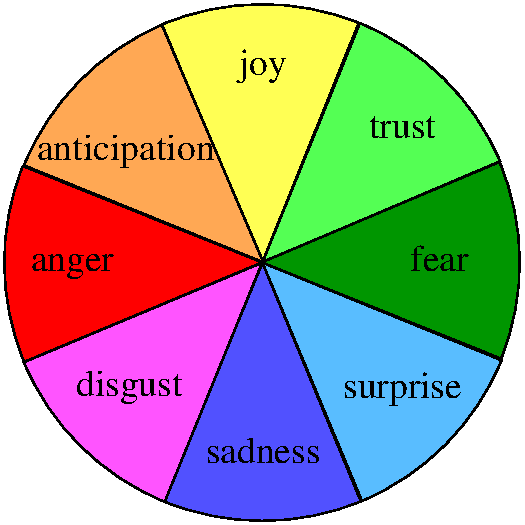
\includegraphics[width = 0.5\linewidth]{figure/plutchikWheel.pdf}
    \caption{Plutchik basic emotions}
    \label{fig:plutchikLabel}
\end{figure}
\begin{align}
    \forall \vec{C} \in \mathbf{D}, \vec{C} &= \begin{bmatrix}
                                                e_{1} \\
                                                e_{2} \\
                                                \vdots \\
                                                e_{8}
                                                \end{bmatrix}, 
    e \in [0, 1]
\end{align}
\noindent Given the context of a story, i.e., all previous sentences $\vec{X} = \{x_1, x_2, x_3, \dots, x_m\}$, the goal is to predict the emotions $\vec{C_i}$ that will appear in the next sentence. 


% Essentially, the model provides the confidence level of each categories $\mathcal{P}(\vec{C_i} | \vec{X}) = \Pi^8_{k=1}\mathcal{P}(c_k | \vec{X})$, which will be transformed into the final result by setting the threshold value to $0.600$. 

For example, for the following input sequence of sentence $\textsc{S}_1$ that serves as context, the model may predict the emotions in the next sentence to be \texttt{joy, anticipation, }and \texttt{trust}.

\begin{center}
    \texttt{
    $\textsc{S}_1$: He was hoping this year to be tall enough for the coaster.
    }
\end{center}

%where does 17910 comes from, there is also 1680 in later sections
For preparing the training data, we obtained 17,910 pairs of story context and next-sentence emotions from the Story Commonsense dataset. The dataset was divided into training and validation sets in the ratio of 6:4. We then fine-tuned the BERT$_{\textsc{Next Emo}}$ model %from Huggingface
using the task of multi-label classification. The story context is the input, and the next-sentence emotions are the output. The maximum input length of the tokenizer was set to 120. The batch size was set to 16, and the learning rate was set to $6e-6$. We ran 16 epochs for training, which took about 45 minutes on a Tesla P100-PCIE-16GB GPU. The model achieved a Macro ROC-AUC score of 0.69 on prediction. The prediction results are not perfect. However, they are only used as suggestions, and the user can always overwrite them. 

\subsection{Keywords Extraction}
For training the model and evaluation, we extract keywords from the original five-sentence stories. We used the \texttt{SceneGraphParser()} from~\cite{wu2019unified} to parse sentences (in natural language) into scene graphs. The entities in the scene graphs become the keywords. For example, for the following sentence: 
\begin{center}
    \texttt{
    $\textsc{S}_1$: I brought the movie home and watched the whole thing.
    }
\end{center}
We are expected to generate the following result:
\begin{center}
    \texttt{'I, the movie, the whole thing'}
\end{center}


\section{Initial Result}
We have currently finishing fine-tuing the Teacher Network based on \texttt{Davinci-003}. It is able to provide decent results with qualified performance in various metrics including BLEU and BERT score. As further parameter-tuning is necessary, further results and visualization will be provided in the formal respot.

\section{Future Work and Schedule}

We have used T5 as the pre-trained LLM for our story generation framework. We will explore different techniques for generating narrative structures, such as using knowledge graphs to represent characters and plot elements and controlling the generation process to ensure coherence and consistency. We will also use a fine-tuning approach to adapt the LLM to the task of story generation and improve its performance in generating coherent and engaging stories. Through this process we will derive equations in the knowledge distillation which could have an impact on the framework. We are still determining how we will implement and utilize knowledge distillation graphs.

We expect to develop a framework that can generate coherent and engaging stories with rich narrative structures, including character development, plot progression, and conflict resolution. We also anticipate that our framework will be able to generate stories that are engaging and can be enjoyed by a wide audience. Furthermore, we expect to identify the most effective techniques for narrative structure generation and fine-tuning the LLM for story generation. Ultimately, we are on schedule to make significant progress on our project by the April 20th due date. We intend to finish most of the work beforehand to allow time to develop the final research paper and the presentation.

\bibliography{bib}
\bibliographystyle{aaai}

\end{document}